\documentclass[tikz]{standalone}

\usepackage[T1]{fontenc}
\usepackage[english]{babel}

\usepackage{standalone}

\usepackage{tikz}
\usetikzlibrary{calc}

\begin{document}
    \begin{tikzpicture}
        \node (3d) at (0,0) {
            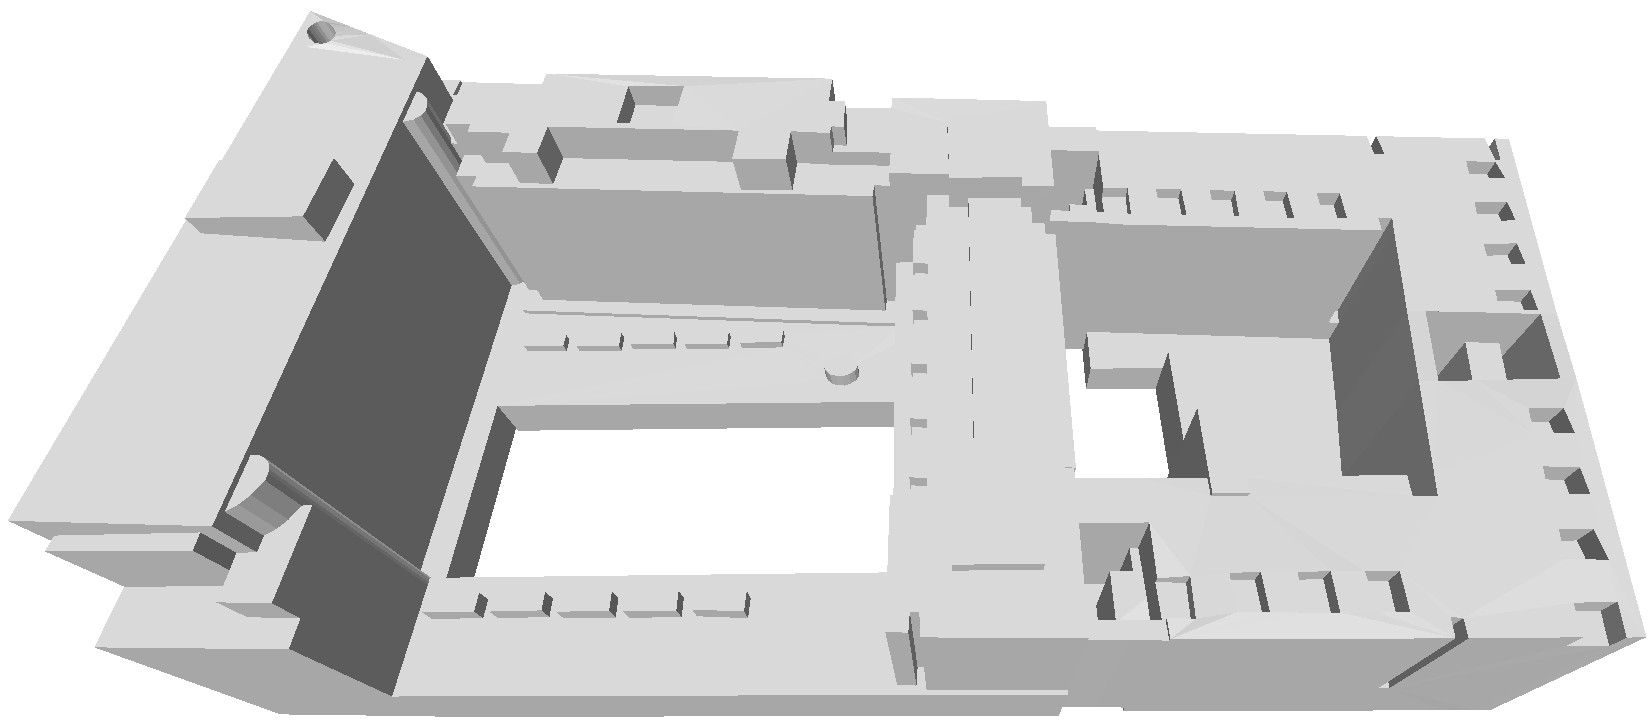
\includegraphics[height=4cm]{images/difference_mesh_model/ground_truth}
        };
        \path (3d) + (-2, -1.5) node (facet_point) {};
        \path (3d) + (1, -2.25) node[orange] (facet) {\scriptsize Facet $\equiv$ architectural feature};
        \path ($(facet.west) ! .8 ! (facet_point)$) node (halfway_facet_point) {};
        \path[draw, ->, orange] (facet.west) -- (halfway_facet_point |- facet.west) -- (facet_point);
        \path[draw, blue, line width=0.5mm] (-1, 2)  -- (1, 2) node [midway, below] {\tiny \SI{50}{m}};
        \path[draw, blue, line width=0.1mm] (-1, 2)  -- (-1, 2.1);
        \path[draw, blue, line width=0.1mm] (1, 2)  -- (1, 2.1);        
    \end{tikzpicture}
\end{document}
